\documentclass[fleqn,10pt]{wlscirep}
\usepackage[utf8]{inputenc}
\usepackage[T1]{fontenc}
\usepackage{algorithm,algpseudocode}
\usepackage{mathtools}
\DeclarePairedDelimiter\ceil{\lceil}{\rceil} 
\title{Pattern matching based denoising for images with repeated sub strucutures.}

\author[1,*]{Alice Author}
\author[2]{Bob Author}
\author[1,2,+]{Christine Author}
\author[2,+]{Derek Author}
\affil[1]{Affiliation, department, city, postcode, country}
\affil[2]{Affiliation, department, city, postcode, country}

\affil[*]{corresponding.author@email.example}

\affil[+]{these authors contributed equally to this work}

%\keywords{Keyword1, Keyword2, Keyword3}

\begin{abstract}
Example Abstract. Abstract must not include subheadings or citations. Example Abstract. Abstract must not include subheadings or citations. Example Abstract. Abstract must not include subheadings or citations. Example Abstract. Abstract must not include subheadings or citations. Example Abstract. Abstract must not include subheadings or citations. Example Abstract. Abstract must not include subheadings or citations. Example Abstract. Abstract must not include subheadings or citations. Example Abstract. Abstract must not include subheadings or citations.
\end{abstract}
\begin{document}

\flushbottom
\maketitle
% * <john.hammersley@gmail.com> 2015-02-09T12:07:31.197Z:
%
%  Click the title above to edit the author information and abstract
%
\thispagestyle{empty}

\noindent Please note: Abbreviations should be introduced at the first mention in the main text – no abbreviations lists. Suggested structure of main text (not enforced) is provided below.

\section*{Introduction}

Transmission Electron Microscopy (TEM) imaging has been helpful to solve numerous scientific questions in life and material sciences \cite{CURRY200691}$^{,}$\cite{WANG2008395} . However, at times the noise in the acquired images corrupt the signal beyond a useful level. Noise in images can appear due to intrinsic reasons like problems in the sensors or the digital circuits, or due to external factors like the environment. Image denoising plays a vital role especially in suppressing microscopy image noise.

In TEM, when high energy electron beams interact with the specimen, some rays are absorbed. The quantity of radiation absorbed by the specimen in unit time is called dose rate. For obtaining high resolution images of the specimen, the specimen has to be exposed to the radiation for a long period of time. Hence, a higher dose rate is required. Often, the specimen under examination consists of biological samples or delicate materials. A high dose rate on such samples can destroy the specimen under examination. Low dose rate results in a low signal-to-noise ratio, thus resulting in a noisy image of the specimen. These noisy images are not always useful for further analysis, since the information in images is hard to interpret. Therefore after image acquisition, numerical processing is required to enhance the quality of the image so that it can be used for further analysis. 

Various image denoising algorithms were proposed in the past. Conventional denoising methods  \cite{bcm_nlm}$^{,}$ \cite{DBLP:journals/tip/BM3D} use only noisy images for the denoising task, where as most modern methods involving a deep neural network \cite{zhang2018ffdnet}$^{,}$ \cite{zhang2017beyond} require clean images as ground truths for training. Since clean X-ray and electron microscopy images are not available in most cases, modern denoising methods that require clean images as ground truths cannot be used. However, there are also some deep neural network based methods that use noisy supervision \cite{DBLP:journals/corr/abs-1803-04189} and self supervision\cite{krull2019noise2void}. Although, conventional and self supervised methods have shown success in denoising images, these methods improved the denoising quality only by a small margin for images with repeated patterns (\textbf{see Results}). Hence, a new denoising algorithm is proposed and its results are analyzed and compared with the state of the art methods. 

\section*{Proposed method}

The proposed denoising algorithm identifies similar sub structures within an image at different regions and averages them to suppress the noise. Averaging patches with similar information suppresses noise that is randomly distributed. Since the noise is assumed to be having zero mean, it cancels out when multiple patches are averaged. However the base signal remains the same throughout and averaging does not disrupt the signal. Hence combining different patches results in denoised pixels close to the actual signal value. 

Let $x_{i}$ be the $i^{th}$ noisy patch, $k$ be the number of patches that are averaged, $s_i$, and $n_i$ be the signal and noise in the $i^{th}$ patch respectively. Then,
\begin{equation}
	x_i = s_i + n_i
\end{equation}
Averaging over $k$ patches results in an expected value,
\begin{equation}
	E[\frac{1}{k}\sum_{i}^{k}x_i ] = E[\frac{1}{k}\sum_{i}^{k}(s_i + n_i) ]
\end{equation}
Since the noise is expected to be having zero mean and the base signal is expected to be the same,
\begin{equation}
	E[\frac{1}{k}\sum_{i}^{k}n_i ] = 0
\end{equation}
\begin{equation}
	E[\frac{1}{k}\sum_{i}^{k}s_i ] = s
\end{equation}
since $s_i$ = $s$ for all $i$. Ideally this means that,
\begin{equation}
	E[\frac{1}{k}\sum_{i}^{k}x_i ] = s
\end{equation}
Hence the variance of the averaged patch is small, i.e,
\begin{equation}
	Var[\frac{1}{k}\sum_{i}^{k}x_i ] = \frac{1}{k^2 -1} \sum_{i}^{k}Var(n_i)
\end{equation}
since $Var(s_i) = 0$ for all $i$. Hence averaging patches with the same signal suppresses noise.

%The basic idea of the algorithm can be compared with the Single Particle Imaging \cite{bhushan_single_2017}, which is an image processing technique used to analyze low dose Transmission Electron Microscopy (TEM) images of identical but dose sensitive samples. Images of specimens obtained from TEM are often very noisy, and hence it is difficult to interpret the information contained in the image. Averaging several images of the same specimen can remove random noise and make the information more interpretable \cite{bhushan_single_2017}.

%It can also be said that this algorithm is similar to the Non-Local Means \cite{bcm_nlm} algorithm in some aspects. In Non-Local Means, similar patches are found only from the immediate surroundings, where as the region of interest is not restricted in the proposed denoising algorithm. Increasing the search space in Non-Local Means has a massive impact on the computation speed. 

\subsection*{Outline of the proposed algorithm}
  
The denoising algorithm uses cosine similarity for matching patches. Cosine similarity is a measure that is used to quantify similarities between two vectors \cite{alake_understanding_2021} by finding the cosine of the angle between them. If the vectors are in the same direction (i.e., similar), cosine similarity is maximal. Cosine similarity is also defined as the normalized dot product of the two vectors. It is mathematically represented as,
\begin{equation}
	similarity = cos(\theta) = \frac{A\cdot B}{\|A\|\|B\|} = \frac{\sum_{i=1}^{n}A_i B_i}{\sqrt{\sum_{i=1}^{n}A_i^2}\sqrt{\sum_{i=1}^{n}B_i^2}}
\end{equation}
where $A$ and $B$ are two vectors, and $\theta$ is the angle between them. The cosine similarity value lies between 0 and 1. Normalized convolution between a \textit{reference patch} and an image results in local cosine similarity similar to the result obtained by template matching (Figure \ref{fig:template_matching} demonstrates the working of the template-matching algorithm). An image, a template taken from the image (i.e., \textit{reference patch} in this algorithm), and the corresponding result have been shown. The maximum value in the result which is marked in red, represents the template’s location in the image. It corresponds to the top-left corner of the template. Values close to the maximum represent the patches similar to the template. Hence cosine similarity can be used to match patches with images, similar to template matching. 

\begin{figure}
	\centering
	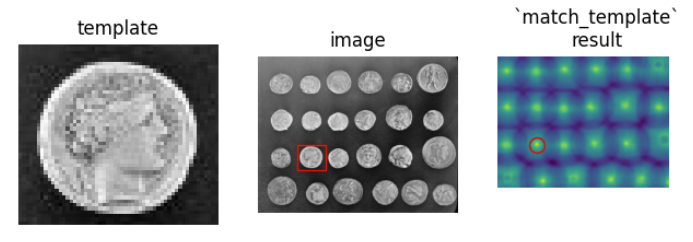
\includegraphics[scale=0.8]{./imgs/template_matching.png}
	\caption[Template matching example]{Template matching example \footnotemark }
	\label{fig:template_matching}
\end{figure} 

The time complexity of the convolution operation is $O(m^2n^2)$, where $m*m$ is the size of the patch and $n*n$ is the size of the image, which is for large $m$ worse than the run-time of the template matching algorithm. Complexity of the template matching algorithm is $O(n^2log(n^2))$ \cite{template_matching}, where $n*n$ is the image size. Since the convolution operation is widely used in convolutional neural networks, there are Python libraries that support GPU computation for performing the convolution operation. Running the computations on the GPU makes the algorithm much faster.

\begin{figure}
	\centering
	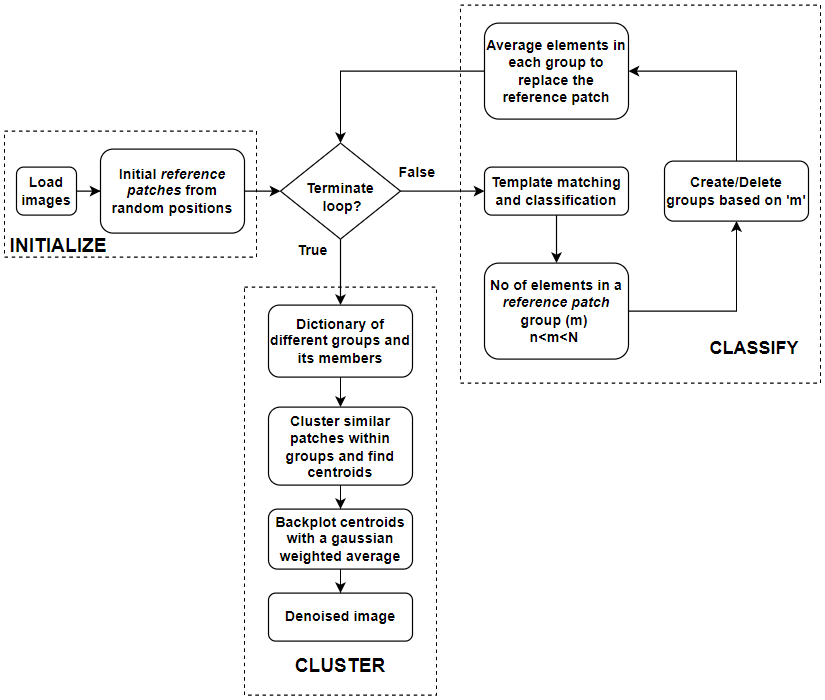
\includegraphics[scale=0.7]{./imgs/flowchart.png}
	\caption{Flowchart of the algorithm}
	\label{fig:flowchart}
\end{figure} 

The proposed algorithm uses the concept of convolution and clustering to perform the denoising task. The flowchart of the algorithm is shown in figure \ref{fig:flowchart}.

The algorithm begins with the initialization of random patches of size $m*m$, which are used for matching other patches of size $m*m$ in the image. The patches that are used as templates for matching are referred to as \textit{reference patches}. For example, initial \textit{reference patches} can be as shown in figure \ref{fig:initial_reference_patches}. The initial \textit{reference patches} ideally should represent different reoccurring regions of an image. Hence, even though the initialization is random, it is ensured that the initial \textit{reference patches} are spread across the image.

\begin{figure}
	\centering
	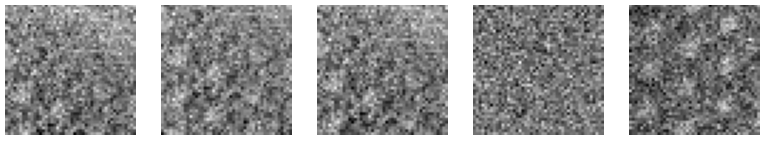
\includegraphics[scale=0.75]{./imgs/initial_reference_patches.png}
	\caption[Initial \textit{reference patches}]{Initial \textit{reference patches} (of size 46*46 pixels), taken from different regions of the input image}
	\label{fig:initial_reference_patches}
\end{figure} 



\footnotetext{\url{https://scikit-image.org/docs/dev/auto_examples/features_detection/plot_template.html}}

In the ``classify” section shown in figure \ref{fig:flowchart}, the patches at every position in the image are classified into different groups based on the cosine similarity values, and these groups are represented by a \textit{reference patch}. If $x$ and $y$ represent a pixel location, then the patch at $(x, y)$ is obtained from pixel locations ($x$ to $x + m$, $y$ to $y + m$), where $m*m$ is the patch size. When the cosine similarity is applied, each of such $m*m$ patches in the image is compared with every $m*m$ \textit{reference patch}. For an image of size $p*q$ and a \textit{reference patch} of size $m*m$, the cosine similarity result has a size $(p - m + 1)*(q - m + 1)$. The result has values between 0 and 1 as the results are normalized. The location with a perfect match is represented by value 1. The patches similar to the \textit{reference patch} are represented by values close to 1. 

Cosine similarity is carried out with $n$ \textit{reference patches}. The result for each \textit{reference patch} is of shape $(p - m + 1)*(q - m + 1)$. All results are stacked into an $n * (p - m + 1)*(q - m + 1)$ array. From this array, the \textit{reference patch} that matches the best at every location is identified. Hence, the $n * (p - m + 1)*(q - m + 1)$ array is reduced to a  $(p - m + 1)*(q - m + 1)$ array which contains the best fitting reference patch index at every position. Now, the patches in the image that are most similar to the reference patches are identified  and grouped together.   

%When cosine similarity is carried out with $n$ \textit{reference patches}, result of shape $(p-m+1)*(q-m+1)$ are obtained for each \textit{reference patch}. These results are stacked into an $n*(p-m+1)*(q-m+1)$ array. From this array, the \textit{reference patch} that matches the best at every location is identified. Hence, the $n*(p - m + 1) * (q - m + 1)$ array is reduced to a $(p-m+1)*(q-m+1)$ array which contains the best fitting\textit{ reference patch} index at every position. Now, patches in the image similar to the \textit{reference patches} are identified. The patches represented by the same \textit{reference patch} form a group.

%Although patches at every location are classified to belong into a group, all these patches are not considered. The patches which have a strong correlation with one of the \textit{reference patches} are prioritized. This is done by selecting patches that are close to the maxima in the template matching result. When these patches with strong correlation are selected, the patches around them in the close neighborhood are deleted. That is, if a patch is selected from $(x, y)$, then no patches in the region from $(x-a$ to $x+a, y-a$ to $y+a)$ are selected, where $(a \approx m/4)$ with $m*m$ being the patch size. This gap between patches is used to remove redundant information. Removing redundant information improves the computation speed without affecting the denoising quality.

In the next step, the newly formed groups are deleted or split into more groups based on the group size. The reasoning behind this process is that groups with few members contribute hardly to any denoising, while overly large groups might lead to a loss of detail.  Finally, for each group the old \textit{reference patch} is replaced by the average of all the members in that group. In the next iteration, cosine similarity and the classification steps repeat with these new \textit{reference patches}. We choose to terminate the “classify” section when the total number of reference patches in three consecutive iterations remains the same. Figure \ref{fig:final_reference_patches} shows the reference patches generated after 15 iterations. On comparing figure 1 and figure 4, one can observe that the noise in the final reference patches has been significantly suppressed.

%Once groups of similar patches are formed, the groups are deleted or split into more groups based on the member size. This is because that if the group size is small, there is hardly any denoising effect. On the other hand, if the group size is too big, there can be artifacts generated during averaging due to increased variance. Each of the old \textit{reference patches} is now replaced by the average of all the members in that group. In the next iteration, cosine similarity and the classification steps repeat with these new \textit{reference patches}. One can observe that every iteration may generate new \textit{reference patches}. New \textit{reference patches} are generated when big groups are split into smaller groups. The ``classify” section terminates when the total number of \textit{reference patches} in three consecutive iterations remains the same. Figure \ref{fig:final_reference_patches} shows the \textit{reference patches} generated after 15 iterations. On comparing figure \ref{fig:initial_reference_patches} and figure \ref{fig:final_reference_patches}, one can observe that the noise in the final \textit{reference patches} has been suppressed.

\begin{figure}
	\centering
	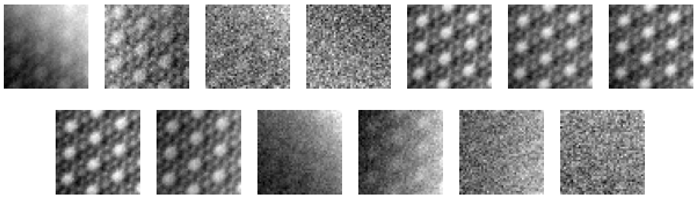
\includegraphics[scale=0.8]{./imgs/final_reference_patches.png}
	\caption{Final \textit{reference patches}}
	\label{fig:final_reference_patches}
\end{figure} 

If the final \textit{reference patches} are used for back plotting (i.e. to replace the patches in their corresponding groups), there are still some artifacts (as shoown ) present because of the following reasons. 

%After running the ``classify” section multiple times, the final \textit{reference patches} are used to replace the patches in their corresponding groups. The denoised image is constructed by using these final \textit{reference patches}. Since \textit{reference patches} can overlap during reconstruction, a $2D$ Gaussian weight is used. The information at the center of a patch is important than the edges. While back plotting, if multiple patches overlap, a weighted average is done. Weighted average with Gaussian weights ensures that the back plotted images do not have sharp edges from the patches used, as the information from the patch edges is suppressed. The back plotted image can be seen in figure \ref{fig:backplot-1}. The following can be inferred from the back plot:

\begin{itemize}
	\item There can be patches in a group that are less similar to the \textit{reference patch}. When these dissimilar patches are averaged, the average might differ from the actual patch by a large extent. 
	\item Averaging a large range of data also changes the range of pixel values,
	altering the brightness after reconstruction.
\end{itemize}

These problems can be solved by averaging over a small group with very closely matched patches. Clustering is applied within every group (represented by the final \textit{reference patch}) to create smaller subgroups, i.e., clusters are created within large groups. The number of clusters in a group, is obtained by dividing the number of patches in a group by `$c^2$’, where $c$ is user defined. In other words, the signal-to-noise ratio can be adjusted by changing the `$c$’ value. The centroids found from clustering now represent a large group that was before represented by a single \textit{reference patch}.  Centroids used for back plotting are multiplied by a $2D$ Gaussian weight. A weighted average is performed when more than one centroid is used at a position. Gaussian weight smoothens the edges of the centroids, thus preventing artifacts in the reconstructed image. 

The denoising algorithm can be seen in the section \ref{algorithm:denoising_algorithm}. The implementation of the denoising algorithm can be found on github\footnote{\url{https://github.com/mbanil/img-denoiser}}.

\subsection*{Parameters of the algorithm and stability}

The following are the algorithm parameters.

\begin{itemize}
	\item \textbf{Size of the patches}: Patches represent features in an image. Patch sizes should neither be too small nor too large. A patch size of $46*46$ performed the template matching task reasonably well, and hence this was the size used for most of the experiments. 
	
	\item \textbf{Position of the initial patches}: The position of the initial \textit{reference patches} has to be selected such that the patches represent different regions in the image. These dissimilar patches are selected by randomly initializing the templates such that no two templates are close to each other.
	
	\item \textbf{Minimum number of patches in a group}:  When there are very few patches, averaging them will not significantly suppress the noise. Hence groups with members lesser than this value are deleted.
	
	\item \textbf{Maximum number of patches in a group}: The maximum number of patches in a group (represented by a \textit{reference patch}) is set to 100. The first reason is to avoid over-generalization. If the group size is big, a single \textit{reference patch} will represent too many patches, which is undesirable. 
	
	More groups are generated if this parameter has a lower value, resulting in more \textit{reference patches}. The number of \textit{reference patches} is proportional to the number of times the cosine similarity is applied. Too many \textit{reference patches} can affect the overall computation speed of the algorithm. Hence a trade-off is required.
	
	\item \textbf{The number of clusters within a group}: This parameter must be set based on how much self-similarity is present in the input image. If there is much self-similarity, few clusters can be made because more patches are very close to each other. Hence a centroid can be used to represent more patches. If there is not much self-similarity, more clusters are required to group more similar patches. Hence, this parameter depends on the level of self similarity in the input image. 

\end{itemize}

\section*{Results}

The proposed algorithm is mainly developed to denoise TEM images with repeated structure. An example of such an image and it's denoised result can be seen in figure \ref{fig:denoised_result-1}. For our experiments, a patch size of 46*46, a group size was between 4 and 100, and the clustering parameter $c$ equal to 2.7 were used.

Peak Signal-to-Noise Ratio (PSNR) and Structural Similarity Index Measure (SSIM) are commonly used to measure the quality of image denoising. Both of these techniques required an original noise-free image to calculate the quality of denoising. Since an original noise-free image is not present for the experimental data used, Fast Fourier Transform (FFT)\footnote{\url{https://numpy.org/doc/stable/reference/generated/numpy.fft.fft2.html}} of the image is used to examine the quality of denoising. 

The FFT converts data from the spatial domain into the frequency domain. The white structures in the FFT represent the information in the images. The signal corresponding to the low frequency components are represented at the center of the FFT and higher frequency components are present as we move away from the center. Noise corresponds to the high frequency components of the FFT and is present close to the edges. 

Figure \ref{fig:comparison} shows a comparison of different results. Noisy image, it's FFT, denoised images from different methods and their FFT's can be seen.

\subsection*{Comparison of results}

\label{sec:comparison}

\begin{figure}
	\centering
	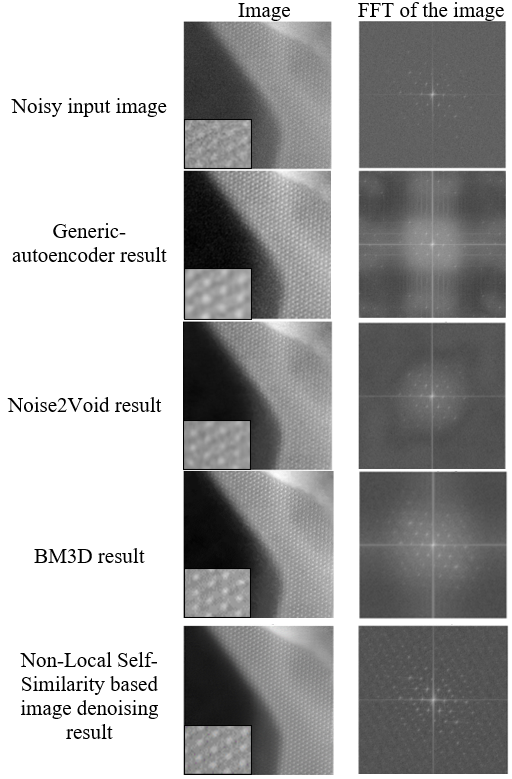
\includegraphics[scale=1.1]{./imgs/comparison-1.png}
	\caption{Comparison of results obtained from different methods}
	\label{fig:comparison}
\end{figure}

The noisy image, the results from all the methods and their Fourier transforms can be seen in figure \ref{fig:comparison}. The result from the generic autoencoder looks a bit noisy even though the circular structures are prominently visible than it's noisier counterpart. The substructures between the circular structures are not visible. The black region also looks noisy. The Fourier transform supports this argument as there isn't any remarkable enhancement in the white structures at the center. The edges appear bright which can be attributed to the noise still existing or additionally added by the denoising process.



N2V does a good job in reconstructing the circular structures and removing the noise in the black region. However, the substructures have not been reconstructed well. The Fourier transform shows that the enhancement of white structures at the center. The edges mostly look dark thus representing the suppression of noise. 

BM3D does a slightly better job than N2V. This is also supported by the Fourier transform. However the substructures are not reconstructed well. 

Non-Local Self-Similarity based denoising has produced the best result among the methods that have been tested on the experimental data. This method does a good job in reconstructing most of the structures from the noisy image. The Fourier transform also shows enhancement in the white structures which is the most compared to those from the other methods. Upon observing the result in figure \ref{fig:denoised_result-1_1}, the substructures between the circular structures can also be seen. 


\begin{figure}
	\centering
	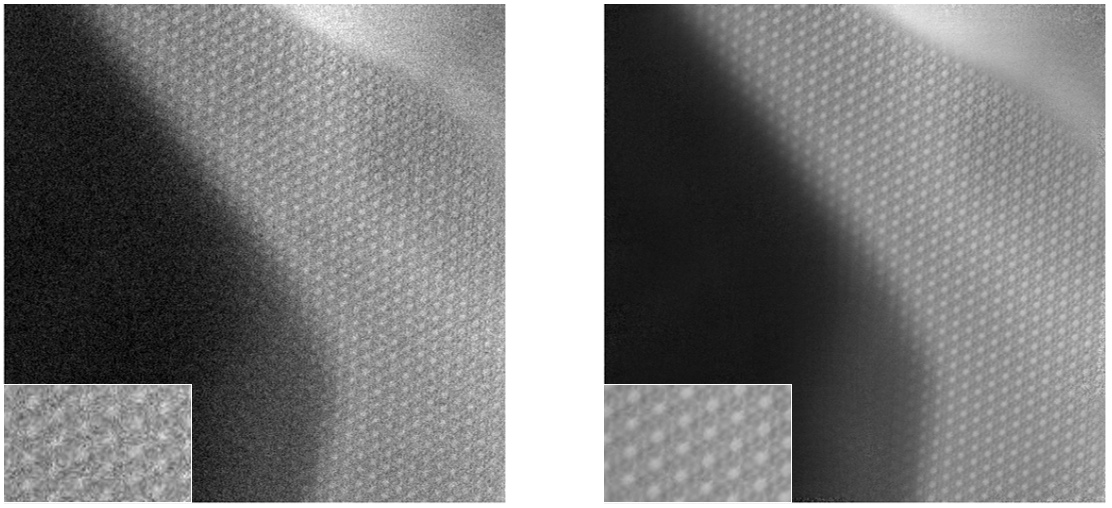
\includegraphics[scale=0.5]{./imgs/denoised_result-1.png}
	\caption[Non-Local Self-Similarity based image denoising result]{Noisy input and it's corresponding denoised result}
	\label{fig:denoised_result-1}
\end{figure}

\begin{figure}
	\centering
	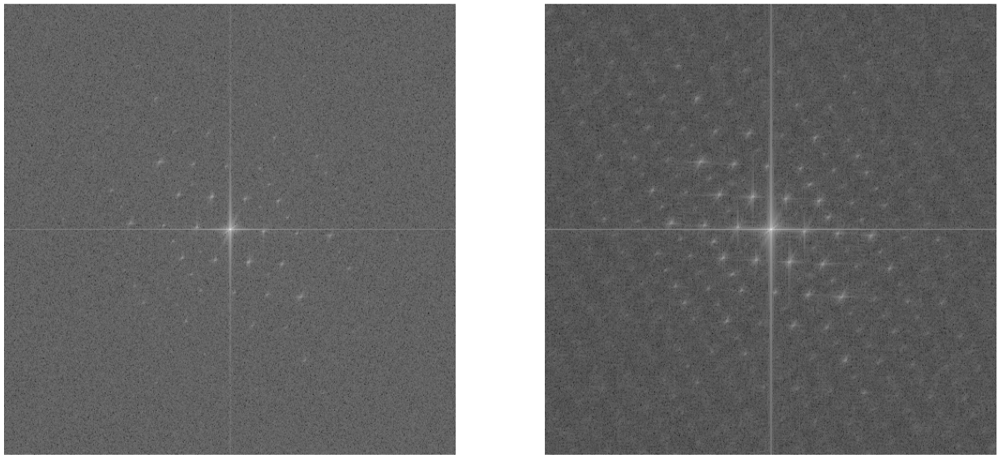
\includegraphics[scale=0.55]{./imgs/denoised_result_fft-1.png}
	\caption[FFT of the Non-Local Self-Similarity based image denoising result]{FFT of the noisy input and it's corresponding denoised result}
	\label{fig:denoised_result_fft-1}
\end{figure}

Peak Signal-to-Noise Ratio (PSNR) and Structural Similarity Index Measure (SSIM) are popularly used to measure the quality of image denoising. Both of these techniques required an original noise-free image to calculate the quality of denoising. Since an original noise-free image is not present for the experimental data used, Fast Fourier Transform (FFT)\footnote{\url{https://numpy.org/doc/stable/reference/generated/numpy.fft.fft2.html}} of the image is used to examine the quality of denoising. 





\subsection*{Noise Suppression}

The main reason for noise suppression is the averaging of very similar patches in the image. Suppression of noise is proportional to $\sqrt{n}$, where $n$ is the number of patches used \cite{bcm_nlm}.

Figure \ref{fig:similar_patches} shows a visualization where each marker represents a patch and same colored markers represent similar patches. It can be observed that each group has many similar patches. As explained in the above paragraph, averaging similar patches will suppress the noise present. Since, sometimes the number of patches in a group can be too large, which leads to problems shown in figure \ref{fig:backplot-1}, clustering is done to make smaller subgroups.

\begin{figure}[H]
	\centering
	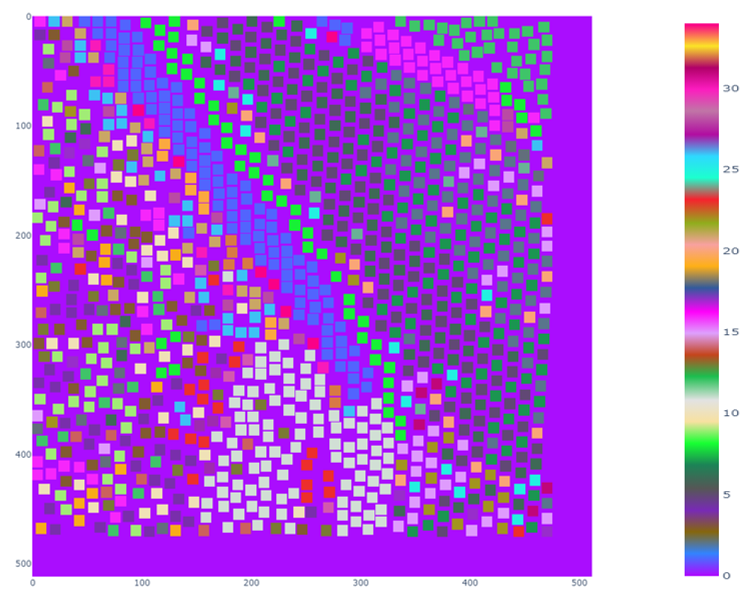
\includegraphics[scale=0.5]{./imgs/similar_patches.png}
	\caption[Visualization of the similar patches in the image]{Visualization of the similar patches in the image. Same colored squares represent similar patches (forming a group) and hence different colors of the squares represent different groups.}
	\label{fig:similar_patches}
\end{figure}

Consider a group of patches that are represented by the same colored squares in figure \ref{fig:similar_patches}. The group members become the samples for clustering, and the number of clusters depends on the parameter `$c$’ that the user can define. There are around 30 groups shown, and hence clustering is done around 30 times. As explained earlier, hierarchical clustering is the clustering method used. The parameter `$c$’ should be chosen based on the extent of self-similarity in the input image. For this particular image shown in figure \ref{fig:denoised_result-1}, a value of 2.7 was used. Upon experimenting, the ideal range for this parameter was between 1.5 (for images with less similar components) and 2.7 (for images with more similar components). The number of clusters in a group is found by,

\begin{equation}
	w = \ceil*{\frac{n}{c^{2}}}
	\label{eq:clustering}
\end{equation}

where $w$ is the number of clusters, $n$ is the number of group members, and $\ceil{}$ represents the conversion to the next highest integer.

\begin{figure}
	\centering
	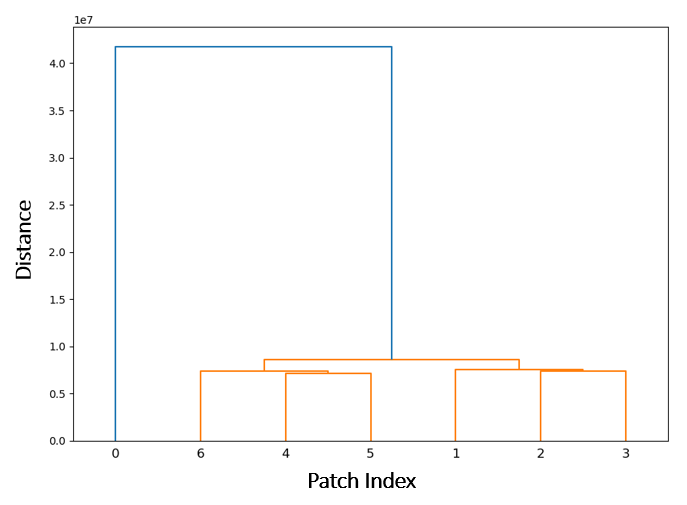
\includegraphics[scale=0.7]{./imgs/bad_clustering.png}
	\caption[Clustering - bad example]{Dendrogram obtained from hierarchical clustering on a group. The group is not split and hence a single cluster is obtained.}
	\label{fig:bad_clustering}
\end{figure}

Sometimes clustering can also fail to create smaller clusters when the clustering parameter is not chosen correctly. In figure \ref{fig:bad_clustering}, there are seven members, and choosing a clustering parameter of 2.7 will result in one cluster, which is not desirable as one of the members is dissimilar from the rest of the group. Clustering parameter having a higher value has an advantage as the noise suppression is more. However, it can introduce some artifacts if there is not much self-similarity in the image. 

Once the different centroids are obtained, they are back plotted to get the denoised image. Centroids overlap while back plotting and are averaged with a $2D$ Gaussian weight. Averaging here further suppresses the noise. The number of patches that are averaged at every pixel location is visualized in figure \ref{fig:visualization of number of patches}. The visualization also considers the number of patches that form a centroid in the clustering process. One can observe that over 200 patches have been averaged at certain regions, which suppresses the noise by over 90\%  (since suppression of noise is proportional to $\sqrt{n}$, where $n$ is the number of patches used \cite{bcm_nlm}.).

\begin{figure}[H]
	\centering
	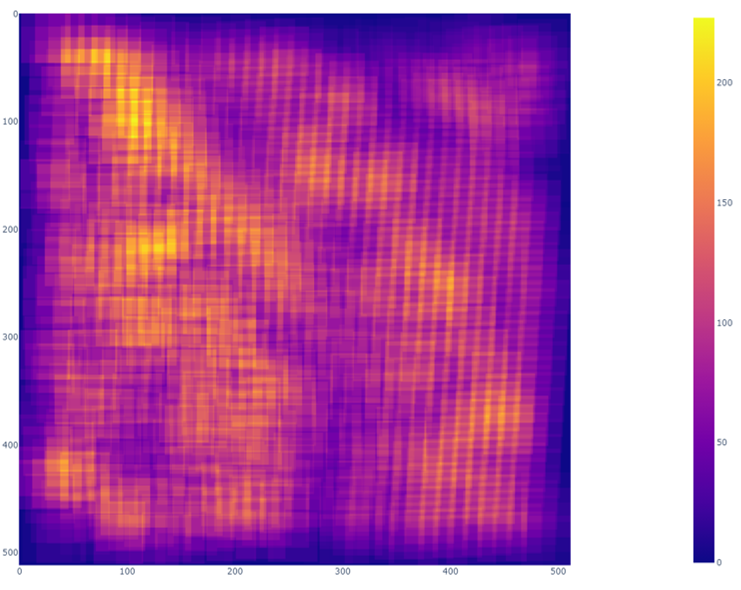
\includegraphics[scale=0.6]{./imgs/visualization of number of patches.png}
	\caption[Visualization of the number of patches averaged at every pixel location]{Each location in the visualization represents the total number of pixels that are averaged at every location to get the denoised result.}
	\label{fig:visualization of number of patches}
\end{figure}

\subsection*{Confidence map}
From the above discussions, it can be observed that the algorithm can introduce artifacts. It is important to recognize this to determine if the denoised image is satisfactory. Since it is challenging to detect minute artifacts from Fourier analysis, a confidence map was developed. This confidence map is based on the variance within each cluster obtained after applying hierarchical clustering. The variance should be small if the centroid is a good representation of its member patches. Also, a good centroid should not have
any patterns in its variance. Patterns in the variance show that the centroid does not generalize its members well. Figure \ref{fig:variance_of_centroid} shows the centroids which is a good generalization (centroid-1) and which is not (centroid-2). The centroid-2 has been taken for demonstration purposes by having very few clusters in a group. 

\begin{figure}[H]
	\centering
	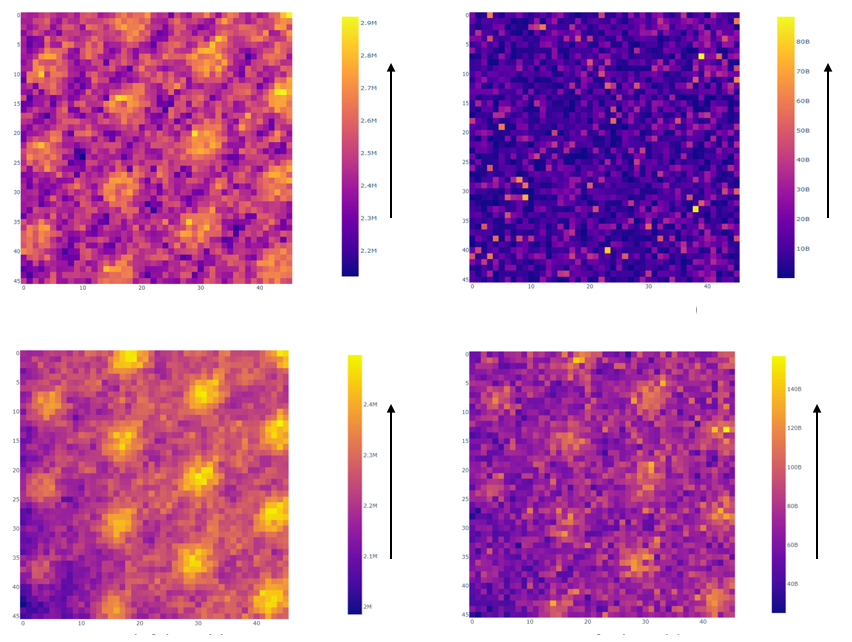
\includegraphics[scale=0.6]{./imgs/variance_of_centroid.png}
	\caption[Centroid and variances of clusters]{Centroid\_1 and variance\_1 in the top row - Variance is low in this case which is desirable. Centroid\_2 and
		variance\_2 in the bottom row - Variance is high and has structures in this case which is undesirable.}
	\label{fig:variance_of_centroid}
\end{figure}

The confidence map of the denoised image is calculated by combining the variances for different centroids as they are back plotted. The algorithm \cite{chan1982updating} for combining the variances has been mentioned in appendix \ref{algorithms} under algorithm \ref{algorithm:variance_algorithm}.

The overall variance map, i.e., the confidence map of a denoised image is as shown in figure \ref{fig:confidence_map}. This result has been produced for demonstration purpose with a very few initial \textit{reference patches} selected very close to each other. The bright regions in the confidence map correspond to the denoised image artifacts. For instance, a bright region can be seen in the confidence map at the top-right position. An artifact can be found by inspecting the same region on the denoised image. Similarly, irregularities in the black region on the left side of the denoised image can be recognized by the brighter regions of the confidence map.

\begin{figure}[H]
	\centering
	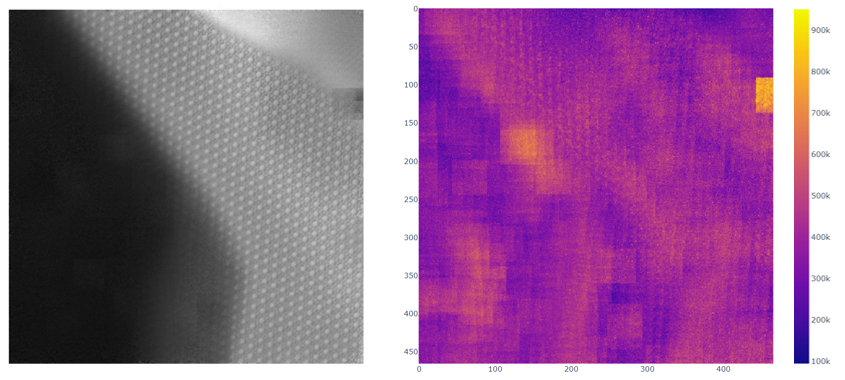
\includegraphics[scale=0.7]{./imgs/confidence_map.png}
	\caption{Denoised image and it's confidence map}
	\label{fig:confidence_map}
\end{figure}

\begin{figure}[H]
	\centering
	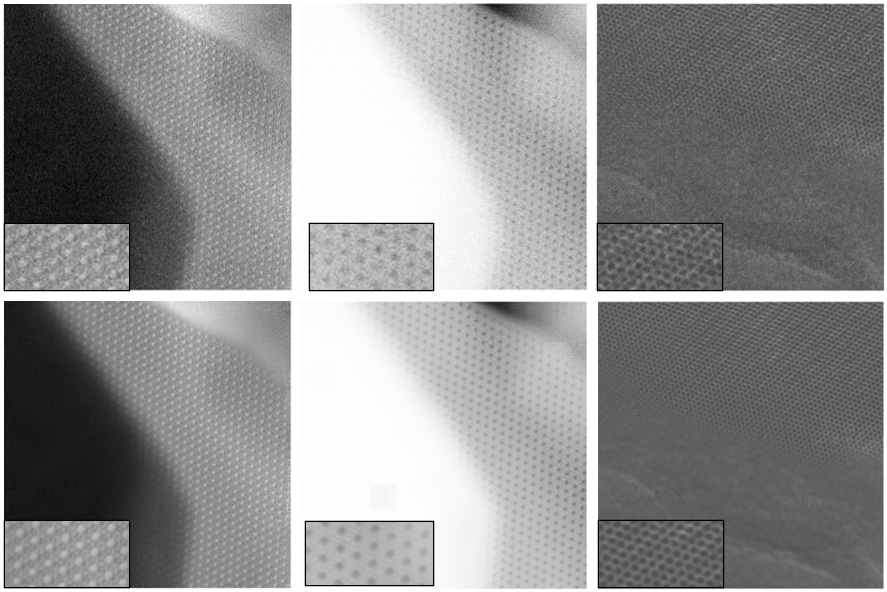
\includegraphics[scale=0.65]{./imgs/denoising_algo_result.png}
	\caption[Non-Local Self-Similarity based image denoising result for all experimental data]{Noisy images in the top row and their corresponding denoised images in the bottom row}
	\label{fig:denoised_result_analysis}
\end{figure}

\subsection*{Other results}

The results of the algorithm for all the experimental images are as shown in figure \ref{fig:denoised_result_analysis}. On inspection, it can be observed that the denoising task has been carried out fairly well, suppressing the noise and enhancing the image features.

\subsection*{Comparision of results}




\subsection*{Subsection}

Example text under a subsection. Bulleted lists may be used where appropriate, e.g.

\begin{itemize}
	\item First item
	\item Second item
\end{itemize}

\subsubsection*{Third-level section}

Topical subheadings are allowed.

\section*{Discussion}

The Discussion should be succinct and must not contain subheadings.
 

\bibliography{sample}

\noindent LaTeX formats citations and references automatically using the bibliography records in your .bib file, which you can edit via the project menu. Use the cite command for an inline citation, e.g.  \cite{Hao:gidmaps:2014}.

For data citations of datasets uploaded to e.g. \emph{figshare}, please use the \verb|howpublished| option in the bib entry to specify the platform and the link, as in the \verb|Hao:gidmaps:2014| example in the sample bibliography file.

\section*{Acknowledgements (not compulsory)}

Acknowledgements should be brief, and should not include thanks to anonymous referees and editors, or effusive comments. Grant or contribution numbers may be acknowledged.

\section*{Author contributions statement}

Must include all authors, identified by initials, for example:
A.A. conceived the experiment(s),  A.A. and B.A. conducted the experiment(s), C.A. and D.A. analysed the results.  All authors reviewed the manuscript. 

\section*{Additional information}

To include, in this order: \textbf{Accession codes} (where applicable); \textbf{Competing interests} (mandatory statement). 

The corresponding author is responsible for submitting a \href{http://www.nature.com/srep/policies/index.html#competing}{competing interests statement} on behalf of all authors of the paper. This statement must be included in the submitted article file.

\begin{figure}[ht]
\centering
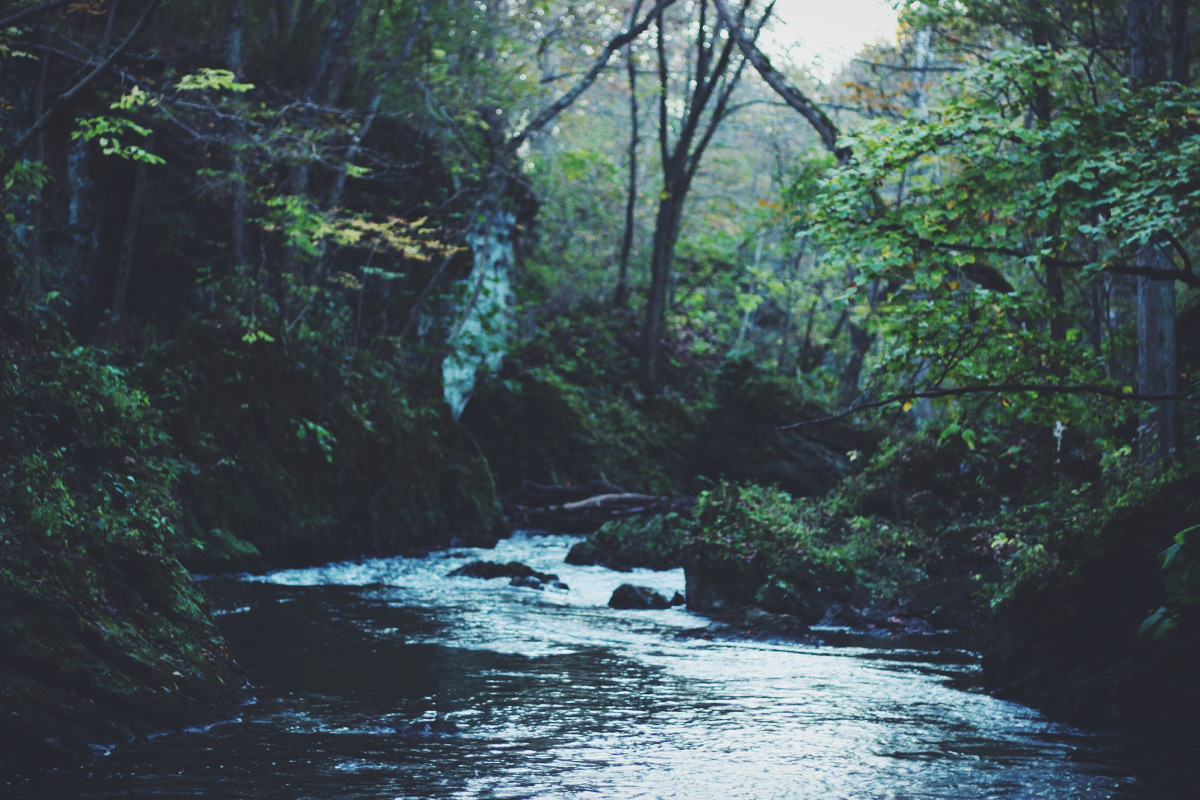
\includegraphics[width=\linewidth]{stream}
\caption{Legend (350 words max). Example legend text.}
\label{fig:stream}
\end{figure}

\begin{table}[ht]
\centering
\begin{tabular}{|l|l|l|}
\hline
Condition & n & p \\
\hline
A & 5 & 0.1 \\
\hline
B & 10 & 0.01 \\
\hline
\end{tabular}
\caption{\label{tab:example}Legend (350 words max). Example legend text.}
\end{table}

Figures and tables can be referenced in LaTeX using the ref command, e.g. Figure \ref{fig:stream} and Table \ref{tab:example}.


\subsection*{Algorithm}
\label{algorithms}

\begin{algorithm}
	\caption{Denoising Algorithm}
	\label{algorithm:denoising_algorithm}
	\begin{algorithmic}[1]
		\State \textbf{Input}: Noisy image
		\State \textbf{Result}: Denoised image
		\State \textit{imgs} $\gets$ loadImgs() ;
		\State set [\textit{templateSize, minGroupSize, maxGroupSize, clustParam}] ;
		\State \textit{refPatches} $\gets$ generate\_initial\_ref\_patches(\textit{imgs}, \textit{templateSize}) ;
		\State \textit{c} $\gets$ 15 ;
		
		\For{\textit{c} $\geq$ 0 \textbf{or} (check if the number of \textit{refPatches} in the last two iterations has changed)}
		
		\State \textit{tmpMatchResult} $\gets$ [ ]	;		
		
		\For{\textit{img} in \textit{imgs}}
		\For{\textit{refPatch} in \textit{refPatches}}
		
		\State \textit{tmpMatchResult}.append(template\_matching(\textit{img}, \textit{refPatch})) ;
		
		\EndFor
		\EndFor
		
		\State \textit{maxValue} $\gets$ max(\textit{tmpMatchResult}, axis=2) ;
		\State \textit{refPatchIndex} $\gets$ `\textit{refPatches}' index at \textit{maxValue} ;
		\State [\textit{sorted\_maxValue, positionX, positionY}] $\gets$ sortWithIdx(\textit{maxValue}); 
		\State \textit{t} = \textit{templateSize} ;
		\State \textit{list[\textit{idx},\textit{posX},\textit{posY}]} = [ ];
%%		\algstore{part1}
	%%\end{algorithmic}
%%\end{algorithm}
%%\begin{algorithm}
%%	\begin{algorithmic}[1]
%%		\algrestore{part1}
		
		\For{each \textit{s,posX,posY} in \textit{sorted\_maxValue, positionX, positionY}}
		\If{\textit{maxValue[posX,posY]} \textbf{not equal} 0}
		\State \textit{maxValue}[\textit{posX: posX}+($t/4$); \textit{posY: posY}+($t/4$)] $\gets$ 0 ;
		\State \textit{idx} $\gets$ \textit{refPatchIndex}[\textit{posX},\textit{posY}] ;
		\State \textit{list}.append([\textit{idx},\textit{posX},\textit{posY}]) ;
		\EndIf
		\EndFor
		
		\State [\textit{count,refPatchID}] $\gets$ count\_patches\_with\_same\_id(\textit{list});
		% \State \textit{max\_ind} = max(\textit{refPatchIndex}) ;
		
		\For{\textit{cnt,ID} in \textit{count,refPatchID}}
		\If{\textit{cnt} $\le$ \textit{minGroupSize}}
		\State \textit{list} $\gets$ delete(\textit{list}, \textit{ID});
		
		\ElsIf{\textit{cnt} $\ge$ \textit{maxGroupSize}}
		
		\State \textit{list} $\gets$ splitGroup(\textit{list}, \textit{ID}, \textit{maxGroupSize});
		
		%\For{\textit{l} in \textit{list}}
		%	\If{list[idx] == ind}
		%		\If{loopCounter == \textit{params}[\textit{maxGroupSize}]}
		%			\State \textit{loopCounter} = \textit{loopCounter} + 1
		%			\State \textit{list}[\textit{idx}] $\gets$ \textit{max\_ind}
		%			\State \textit{max\_ind} $\gets$\textit{ max\_ind} + 1
		%		\EndIf
		%	\EndIf
		%\EndFor
		
		\EndIf
		
		\EndFor
		
		\State \textit{refPatches} $\gets$ average\_patches\_with\_same\_id(\textit{list}) ;
		
		\State \textit{c} $\gets$ \textit{c}-1 ;
		\EndFor
		\State \textit{subGroup}[\textit{centroid, posX, posY}] = [ ];
		\For{\textit{refPatchID} in \textit{refPatches}}
		\State \textit{patches\_with\_sameRef} $\gets$ get\_patches\_with\_same\_id(\textit{list},\textit{refPatchID});
		\State \textit{numClusters} $\gets$ count(\textit{patches\_with\_sameRef})/\textit{clustParam} ;
		\State \textit{subGroup}.append(cluster(\textit{patches\_with\_sameRef, numClusters})) ;
		\EndFor
		\State \textit{gaussianWeight} $\gets$ createGaussianWeight();
		\State \textit{denoisedImg} $\gets$ backPlot(\textit{subGroup}, \textit{gaussianWeight});
	\end{algorithmic}
\end{algorithm}

\clearpage

\begin{algorithm}
	\caption{Algorithm for calculating variance}
	\label{algorithm:variance_algorithm}
	\begin{algorithmic}[1]
		\State \textit{weight} $\gets$ \textit{weightA} + \textit{weightB} ;
		\State \textit{delta} $\gets$ \textit{avgB} - \textit{avgA} ;
		\State \textit{M2} $\gets$ (\textit{M2\_A} + \textit{M2\_B} + $delta^2$ *  \textit{weightA} * \textit{weightB}) / n ;
		\State \textit{Var\_AB} = \textit{M2} / (\textit{n} - 1);
	\end{algorithmic}	
\end{algorithm}

\end{document}